\subsection{Subsystem 1: Processing}

\subsubsection{Subsystem Diagrams}
\begin{figure}[h]
    \centering
    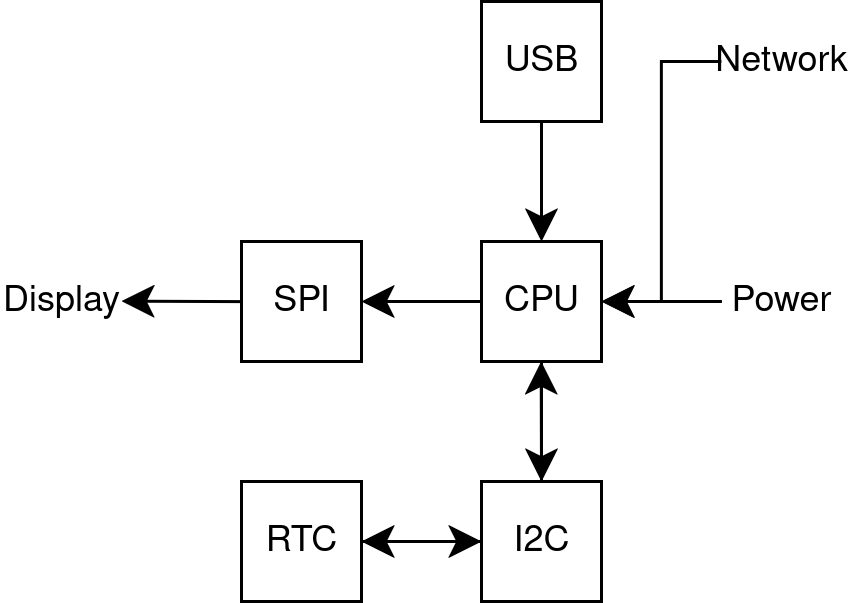
\includegraphics[width=12cm]{images/Processing_Subsystem_Block_Diagram.png} % Change the picture
    \caption{Subsystem Block Diagram}
\end{figure} % If your subsystem is more coding, change it to activity diagram

% Specifications
\subsubsection{Specifications}
\begin{enumerate}
    \item Support SPI clock $\geq$ 20 MHz
    \item SPI support up to 40 MHz, full-duplex, DMA capable
    \item Display update latency $\leq$ 16 ms
    \item Support configurable API refresh interval between 60 and 300 s
    \item API end-to-end fetch latency $\leq$ 2 s
    \item Clock drift $\leq \pm 1\frac{\text{sec}}{\text{day}}$
    \item Operating voltage: $3.3 \pm 0.1$ V
\end{enumerate}

% Subsystem Interactions
\subsubsection{Subsystem Interactions}
The core computer interfaces with
all other subsystems. The battery/power
management unit supplies it with power.
Running processes direct and receive
information from the network module.
It communicates with the digital dot matrix
display via SPI according to display
drivers on the controller.


% Core ECE
\subsubsection{Core ECE Design Tasks}
\begin{itemize}
    \item \textbf{ENGR 16100}: Teamwork \& project documentation.
    \item \textbf{CS 15900}: Fundamentals of programming.
    \item \textbf{ECE 36200}: PCB design and embedded software development.
\end{itemize}

% Parts List
\subsubsection{Parts}
\begin{itemize}
    \item ESP32-S3
    \item DS3231
    \item PCB
\end{itemize}

% Algorithm
\subsubsection{Algorithm}
\begin{lstlisting}
    initialize clock, network, display, location
    DATA = {}

    always 
        wifi keep alive
        error handling
        if power button pressed
            save and shut down
    
    every minute
        update display time

        read ADS-B sensor
        if ADS-B valid
            add to DATA
            if internet connected
                upload ADS-B data
            else
                cache ADS-B data
        else 
            if internet connected
                make API call for flight data
                add to DATA
            else
                add warning ADS-B out of date to DATA
            

        if battery powered
            update battery level in DATA

        update time, weather in DATA
        convert DATA to pixel buffer
        push pixel buffer to displar
    every hour
        sync with network time
        make API call for weather

\end{lstlisting}

\subsubsection{Theory of Operation}
The processing subsystem is responsible for
coordinating all other subsystems and serving
as the “brain” of the Aviator device. At startup,
the ESP32-S3 initializes its real-time clock,
connects to the Wi-Fi network, and
configures the SPI interface for display communication.
During normal operation, the processor maintains a
persistent network connection to ensure timely access
to APIs.

Every minute, the processor updates the displayed time,
retrieves the latest flight information from the network
subsystem, and parses the response into a standardized
data structure. If the device is battery-powered, it
also queries the power management subsystem for voltage
information and appends this to the displayed data.
The processor then converts the compiled information
(time, weather, and flight updates) into a pixel buffer
and transmits it to the display subsystem.

On an hourly basis, the processor synchronizes the
real-time clock with network time servers and fetches
weather data for local context. Error handling
routines ensure that loss of network, corrupted data,
or power fluctuations do not crash the system; instead,
the subsystem retries API calls or falls back to cached
data, with a warning that the data is out of date.

% Specification Measurement
\subsubsection{Specifications Measurement}
[\textbf{DD3+} Every specification here should match the specification above. ]
\begin{enumerate}
    \item {[Copy specification here. ]} \\
          {[Explain the specification here. Add photoes if necessary. ]}
\end{enumerate}

% Standards
\subsubsection{Standards}
\begin{itemize}
    \item \textbf{IPC-2221}: Governs PCB trace width, spacing, creepage/clearance, via rules, grounding, etc.
    \item \textbf{IPC-A-610}: Covers soldering quality and workmanship.
    \item \textbf{RFC 5905}: Protocol for syncing ESP time to internet.
\end{itemize}